\documentclass[a4paper,10pt]{article}

\usepackage[activeacute,spanish]{babel}
\usepackage[utf8]{inputenc}
\usepackage{xcolor}

\usepackage{hyperref}
\usepackage{multicol}
\usepackage{multirow}

\usepackage{graphicx}

\usepackage{float}

\usepackage[shortlabels]{enumitem}

\usepackage{amsmath,amssymb,amsfonts,amsthm,amscd}

\usepackage{tocloft}
\renewcommand\cftsecfont{\color{blue}}
\renewcommand\cftsubsecfont{\color{blue}}

\newcommand{\dotssquare}{\dotfill$\square$}

\DeclareMathOperator{\arccot}{arccot}

\newtheoremstyle{teorema}{18pt}{15pt}{\parskip=0pt\itshape}%
{}{}{}{ }{\textbf{\thmname{#1} \thmnumber{#2}\thmnote{ (#3)}.}}
\newtheoremstyle{plano}{18pt}{15pt}{\parskip=0pt}%
{}{}{}{ }{\textbf{\thmname{#1} \thmnumber{#2}.} \thmnote{(\textit{#3})}}
\newtheoremstyle{titulo}{18pt}{15pt}{\parskip=0pt\itshape}%
{}{}{}{ }{\textbf{\thmnumber{#2}.\thmnote{ #3}.}}


\theoremstyle{teorema}
\newtheorem{teor}{Teorema}[section]
\newtheorem{lema}[teor]{Lema}
\newtheorem{coro}[teor]{Corolario}
\newtheorem{prop}[teor]{Proposición}
\newtheorem{defi}[teor]{Definición}

\theoremstyle{plano}
\newtheorem{ejem}[teor]{Ejemplo}
\newtheorem{ejems}[teor]{Ejemplos}

\theoremstyle{titulo}
\newtheorem{resu}[teor]{Resultado}

\setlength{\parskip}{.5em}
\setlength{\parindent}{.7em}

\newcommand{\todo}{\textcolor{white}{\colorbox{red!70}{fórmula}}~}
\newcommand{\refer}{\textcolor{white}{\colorbox{green!90!blue}{ref}}~}
\newcommand{\struct}{\textcolor{white}{\colorbox{blue!90!red}{estructura}}~}


\author{David Cabezas Berrido}
\title{Taller avanzado de \LaTeX: ejercicio 8}
\date{}

\selectlanguage{spanish}
%\usepackage{showkeys}  %Desbloquear para ver las referencias cruzadas en el documento



\begin{document}

\maketitle

\begin{abstract}
Ejercicios de las sesiones 4 y 5 en un único documento.
\end{abstract}

\tableofcontents

\section{Ejercicio 1: secciones, párrafos y estilo}

%Subsección
\subsection{Tres párrafos normales}

Lorem ipsum dolor sit amet, consectetur adipiscing elit. Cras sagittis tincidunt mauris, nec gravida nunc porta sed. Duis eu ultrices quam. Praesent pulvinar tortor sed leo dignissim lacinia. Pellentesque fermentum leo sed elit sollicitudin eleifend. Aenean placerat ipsum eu orci varius hendrerit. Curabitur condimentum suscipit quam non ornare. Etiam vel lacus mauris. Duis congue turpis ipsum, scelerisque consectetur nunc laoreet ac.

Etiam ultrices metus eu est venenatis ultrices. Pellentesque habitant morbi tristique senectus et netus et malesuada fames ac turpis egestas. Maecenas id convallis neque, at convallis turpis. Donec mollis consequat turpis et pellentesque. Pellentesque ut enim mattis, placerat est a, vehicula lacus. Morbi sodales, massa in venenatis efficitur, eros lectus varius eros, sed egestas magna dolor ac tortor. Suspendisse vel nisl dui. Phasellus congue eros mauris, non tincidunt turpis rhoncus id.

Cras vulputate eros sem, eu laoreet diam pharetra vel. Sed nulla ipsum, lacinia sit amet ullamcorper eget, dictum vulputate urna. Fusce tempor, nibh ut egestas tempus, neque lacus sollicitudin elit, accumsan dignissim eros enim vitae elit. Suspendisse scelerisque rhoncus massa id placerat. In nec interdum urna. Duis interdum cursus augue vitae lacinia. Suspendisse rhoncus augue augue, et molestie sapien ornare ut. Curabitur ut arcu non erat laoreet ultrices. Duis lectus risus, mattis ut volutpat non, lobortis a erat. Duis id eros arcu. Vestibulum vel placerat libero, id blandit ex. In ullamcorper quam ipsum, eu iaculis ipsum commodo ut.

\subsection{Algunos párrafos con formatos especiales}

Este es un párrafo normal.

Este es un párrafo con \textbf{algunas palabras en negrita}.

Este es un párrafo con \emph{algunas palabras enfatizadas}.

{\itshape Este es un párrafo en cursiva con \emph{algunas palabras} enfatizadas}.

Este es un párrafo con \underline{algunas palabras subrayadas}.

Este es un párrafo con \fbox{algunas palabras recuadradas}.

Este es un párrafo con ``algunas palabras entrecomilladas''.

Este es un párrafo con \textsc{Algunas Palabras en Versalitas}.

Este es un párrafo con \texttt{algunas palabras en fuente teletipo}.

Este es un párrafo con\textsubscript{subíndices} y\textsuperscript{superíndices}.

Este es un párrafo con \href{https://www-cs-faculty.stanford.edu/~knuth/}{un enlace a la página de Donald Knuth}.

Este es un párrafo con una nota al pie de página\footnote{¡Soy una nota al pie de página!}.

Este párrafo contiene la fecha de compilación: \today.

Este párrafo contiene guiones (- -- ---) y puntos suspensivos (\ldots)

Este es un párrafo con {\Large algunas palabras muy grandes}.

Este es un párrafo con {\scriptsize algunas palabras muy pequeñas}.

Este es un párrafo con \textcolor{red}{algunas palabras en rojo} y \textcolor{blue}{otras en azul}.

Este es un párrafo con cuatro caracteres especiales: \$, \&, \{ y \}. 

Este párrafo contiene código \verb|\comando{argumento}|.


%Sección
\subsubsection{Algunos párrafos con alineación especial}

\noindent Este es un párrafo sin indentación o sangrado.

Este es un párrafo largo donde se han\\ forzado intencionadamente\\ dos saltos de línea (aunque el resultado es horrible).

Este es un párrafo \hspace{3cm} con 3cm de espacio en blanco.

\hspace{3cm} Y este es otro párrafo con 3cm de espacio en blanco.

\vspace{+0.5cm}

Este es un párrafo con 0.5cm más de espacio con el párrafo precedente.

\vspace{-0.3cm}

Este es un párrafo con 0.3cm menos de espacio con el párrafo precedente.

\begin{flushleft}
Este es un párrafo alineado a la izquierda (nótese la falta de sangrado).
\end{flushleft}

\begin{center}
Este es un párrafo centrado.
\end{center}

\begin{flushright}
Este es un párrafo alineado a la derecha.
\end{flushright}

\section{Ejercicio 2: listas y columnas}

\subsection{La compra para esta semana}

\begin{itemize}
    \item Pan
\item Naranjas
\item Salmón
\item Piña
\item Tomates
\end{itemize}

\subsection{Películas mejor valoradas por los usuarios de \href{https://www.imdb.com/chart/top?ref_=nv_mv_250}{IMDB}}


\begin{enumerate}
\item Cadena perpetua
    \item El padrino: parte I
\item El padrino: parte II
\item El caballero oscuro
\item 12 hombres sin piedad
\end{enumerate}

\subsection{Invitados a la boda (viñetas y relleno de línea)}

\begin{enumerate}[(A)]
    \item Invitados del novio\hfill$\square$
    \begin{enumerate}[label=\fbox{\roman*}]
       \item Familia del novio\dotssquare
       \begin{enumerate}[1.]
           \item Padres del novio \dotssquare
            \item Tíos del novio\dotssquare
            \item Abuelos del novio\dotssquare
       \end{enumerate}
        
        \item Amigos del novio
    \end{enumerate}
    
    \item Invitados de la novia\hfill$\square$
    \begin{enumerate}[label=\fbox{\roman*}]
       \item Familia de la novia\dotssquare
       \begin{enumerate}[1.]
           \item Padres de la novia\dotssquare
            \item Tíos de la novia\dotssquare
            \item Abuelos de la novia\dotssquare
       \end{enumerate}
        
    \item Amigos de la novia\dotssquare
    \end{enumerate}
    \item Invitados comunes\hfill$\square$
\end{enumerate}

Familia de la novia

Padres de la novia
Tíos de la novia
Abuelos de la novia

Amigos de la novia

Invitados comunes


\subsection{Múltiples columnas}

Este es un texto distribuido en tres columnas:

\begin{multicols}{3}

Lorem ipsum dolor sit amet, consectetur adipiscing elit. Cras sagittis tincidunt mauris, nec gravida nunc porta sed. Duis eu ultrices quam. Praesent pulvinar tortor sed leo dignissim lacinia. Pellentesque fermentum leo sed elit sollicitudin eleifend. Aenean placerat ipsum eu orci varius hendrerit. Curabitur condimentum suscipit quam non ornare. Etiam vel lacus mauris. Duis congue turpis ipsum, scelerisque consectetur nunc laoreet.

Etiam ultrices metus eu est venenatis ultrices. Pellentesque habitant morbi tristique senectus et netus et malesuada fames ac turpis egestas. Maecenas id convallis neque, at convallis turpis. Donec mollis consequat turpis et pellentesque. Pellentesque ut enim mattis, placerat est a, vehicula lacus. Morbi sodales, massa in venenatis efficitur, eros lectus varius eros, sed egestas magna dolor ac tortor. Suspendisse vel nisl dui. Phasellus congue eros mauris, non tincidunt turpis rhoncus id.

\end{multicols}

Estos son los primeros 25 números primos distribuidos en 5 columnas:

\begin{multicols}{5}
\begin{itemize}
    \item 2
	\item 3
	\item 5
	\item 7
	\item 11
	\item 13
	\item 17
	\item 19
	\item 23
	\item 29
	\item 31
	\item 37
	\item 41
	\item 43
	\item 47
	\item 53
	\item 59
	\item 61
	\item 67
	\item 71
	\item 73
	\item 79
	\item 83
	\item 89
	\item 97
\end{itemize}
\end{multicols}

\section{Ejercicio 3: imágenes, tablas e índice}


\subsection{Imágenes entre el texto}

El ejercicio consiste en introducir las figuras \ref{fig:master}, \ref{fig:font} y \ref{fig:cheque}.

Lorem ipsum dolor sit amet, consectetur adipiscing elit. Cras sagittis tincidunt mauris, nec gravida nunc porta sed. Duis eu ultrices quam. Praesent pulvinar tortor sed leo dignissim lacinia. Pellentesque fermentum leo sed elit sollicitudin eleifend. Aenean placerat ipsum eu orci varius hendrerit. Curabitur condimentum suscipit quam non ornare. Etiam vel lacus mauris. Duis congue turpis ipsum, scelerisque consectetur nunc laoreet ac.

\begin{figure}[h]
    \centering
    
\includegraphics[width=0.5\textwidth]{imagen1}
    \caption{Figura con etiqueta \fbox{\texttt{h}} y 50\% del ancho}
    \label{fig:master}
\end{figure}

Etiam ultrices metus eu est venenatis ultrices. Pellentesque habitant morbi tristique senectus et netus et malesuada fames ac turpis egestas. Maecenas id convallis neque, at convallis turpis. Donec mollis consequat turpis et pellentesque. Pellentesque ut enim mattis, placerat est a, vehicula lacus. Morbi sodales, massa in venenatis efficitur, eros lectus varius eros, sed egestas magna dolor ac tortor. Suspendisse vel nisl dui. Phasellus congue eros mauris, non tincidunt turpis rhoncus id.

Cras vulputate eros sem, eu laoreet diam pharetra vel. Sed nulla ipsum, lacinia sit amet ullamcorper eget, dictum vulputate urna. Fusce tempor, nibh ut egestas tempus, neque lacus sollicitudin elit, accumsan dignissim eros enim vitae elit. Suspendisse scelerisque rhoncus massa id placerat. In nec interdum urna. Duis interdum cursus augue vitae lacinia. Suspendisse rhoncus augue augue, et molestie sapien ornare ut. Curabitur ut arcu non erat laoreet ultrices. Duis lectus risus, mattis ut volutpat non, lobortis a erat. Duis id eros arcu. Vestibulum vel placerat libero, id blandit ex. In ullamcorper quam ipsum, eu iaculis ipsum commodo ut.

\begin{figure}[t]
    \centering
    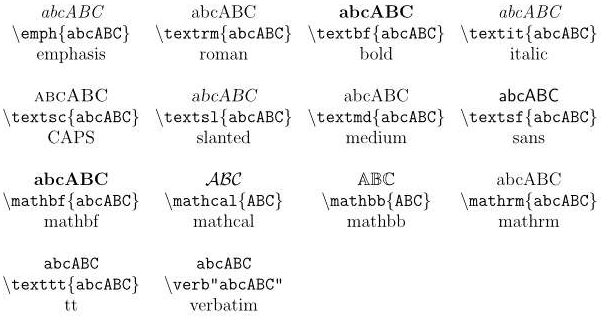
\includegraphics[width=0.8\textwidth]{imagen2}
    \caption{Figura con etiqueta \fbox{\texttt{t}} y 80\% del ancho}
    \label{fig:font}
\end{figure}

Praesent a interdum massa, ut finibus dui. Curabitur sodales, quam a luctus tristique, diam ante tincidunt sapien, nec ultricies diam elit eget lorem. Fusce volutpat erat vitae enim suscipit pellentesque. Curabitur in porta diam. Aenean laoreet vel leo sit amet pretium. Nullam tincidunt pulvinar massa, vitae finibus dui vehicula nec. Duis in tortor euismod, feugiat lectus tristique, dignissim ex. Vivamus eu vestibulum massa. Suspendisse pulvinar orci a orci vestibulum sagittis. Maecenas sapien mi, condimentum vel ante a, blandit euismod turpis. Aliquam laoreet ligula quam, et cursus magna accumsan varius. Fusce placerat, urna non vestibulum malesuada, tellus tortor molestie libero, eget fermentum risus turpis eu felis. Duis vitae dui erat. Quisque eleifend dictum ipsum vitae elementum. Praesent lacinia lectus urna, et consectetur sem porttitor a. Vivamus pharetra ipsum eget dignissim convallis.

Donec eget sapien ac leo consequat cursus. Lorem ipsum dolor sit amet, consectetur adipiscing elit. Fusce velit ligula, hendrerit ac dui sit amet, dapibus ornare tellus. Pellentesque in sem a augue tempor consectetur sed eu lacus. Phasellus mollis dictum metus eu finibus. Nam eu imperdiet nunc. Duis tincidunt molestie dignissim. Sed ullamcorper tristique volutpat. Cras ac pharetra elit, at tincidunt ligula. Nulla facilisi. Suspendisse vulputate purus sit amet elit vestibulum, sed lobortis neque laoreet. Quisque varius velit ac posuere fringilla. Donec ullamcorper felis vitae tortor eleifend, a elementum lectus semper. Vestibulum tincidunt ornare turpis, id venenatis tellus lobortis eget.

Ut nec placerat enim. Praesent interdum ullamcorper tellus id congue. Nullam id tellus neque. Integer at ante feugiat, eleifend felis at, interdum felis. Cras vel sapien arcu. Aliquam in massa eu augue efficitur lacinia ut luctus sapien. Pellentesque vel mi interdum, pulvinar libero sed, pretium velit. Proin auctor, nibh sit amet dictum molestie, ante quam suscipit diam, non scelerisque magna felis quis mauris.

Nunc vitae nulla tellus. Nam tempor lacus ligula, nec tempus diam ullamcorper efficitur. Sed vitae fringilla eros, nec venenatis sem. Proin eu mauris ligula. Integer accumsan sem sed eros pharetra, nec eleifend nibh volutpat. Cras id sapien id leo suscipit auctor. Aliquam accumsan nisl vitae vestibulum posuere. Curabitur vitae varius elit. Sed tempus magna eros, efficitur mattis elit posuere posuere. Interdum et malesuada fames ac ante ipsum primis in faucibus. In hac habitasse platea dictumst. Integer vehicula dignissim volutpat. Aenean est elit, tempor ut tellus vel, malesuada viverra neque. Nullam tempus varius felis eleifend rhoncus. Nullam sapien enim, bibendum sollicitudin mi vel, blandit ultrices erat. Etiam vulputate quam non lobortis rhoncus.

\begin{figure}[b]
    \centering
    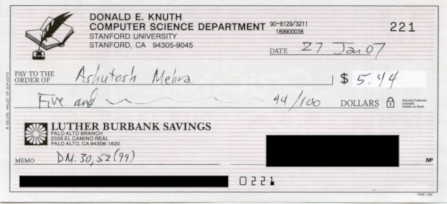
\includegraphics[width=0.7\textwidth]{imagen3}
    \caption{Figura con etiqueta \fbox{\texttt{b}} y 70\% del ancho}
    \label{fig:cheque}
\end{figure}


Etiam imperdiet lorem at dapibus tincidunt. Donec dignissim, sem ac mattis ornare, tellus erat varius sem, eget porta eros est eu elit. Vestibulum tellus nisl, varius a lacus quis, maximus porta sapien. Morbi ultricies id justo vitae vulputate. Pellentesque eros lorem, malesuada nec neque quis, convallis laoreet dolor. Vivamus nibh dui, placerat sed dapibus ac, dignissim eget nibh. Curabitur sed augue vitae quam vulputate suscipit. Nam dignissim magna eget dolor malesuada, facilisis egestas lectus blandit. Proin commodo diam a est feugiat rutrum. In nulla urna, dictum sed lorem eu, varius molestie enim. Phasellus tincidunt ultricies magna, sed facilisis arcu. Vestibulum hendrerit ultricies elementum. Ut vel nisl a nulla congue pretium.

Vestibulum ac nulla tristique erat aliquam vestibulum a nec purus. In dignissim lorem felis, et luctus leo gravida vel. Duis sagittis, mauris at consectetur porta, tortor nibh vehicula risus, id tristique tortor augue porta est. Cras sed vulputate lectus. Aliquam nulla dolor, porta laoreet massa ut, blandit ornare odio. Ut vulputate tellus nec elit dictum, ac condimentum sem auctor. Duis laoreet, neque aliquam commodo euismod, purus lectus placerat elit, a fringilla sapien diam in velit. Quisque blandit odio lacinia commodo lacinia. Aliquam magna elit, venenatis tristique pharetra a, bibendum consectetur mauris. Sed sapien nulla, fringilla at nunc nec, venenatis mollis nulla. Nullam velit turpis, varius et convallis sit amet, cursus gravida velit. Curabitur a venenatis elit. Ut varius est at molestie volutpat. Nullam ut mollis quam, nec volutpat sapien. Curabitur imperdiet pellentesque lectus a dictum. Aliquam ac iaculis ipsum, sit amet consequat risus.

Pellentesque tristique lacinia volutpat. Phasellus vehicula pretium quam, ornare faucibus enim condimentum tempus. Orci varius natoque penatibus et magnis dis parturient montes, nascetur ridiculus mus. Fusce id molestie sapien. Donec tortor metus, placerat id lacus nec, egestas auctor erat. Proin eu erat viverra leo mollis laoreet faucibus eu justo. Cras vel elit at orci pulvinar convallis molestie a magna. Maecenas pretium tortor at mi hendrerit, id ultricies magna blandit.

Sed tincidunt lectus ac lobortis consectetur. Maecenas a dui dapibus, auctor ligula ac, tempus dolor. Aliquam sapien odio, sagittis sit amet justo nec, ornare tincidunt sapien. Nulla leo massa, molestie sed sagittis eget, ultricies non purus. In gravida venenatis velit, vitae cursus augue mollis eu. Vivamus id gravida lectus. Suspendisse vel consectetur urna, ac interdum orci. Cras ac rhoncus nibh, nec pharetra velit. Nullam nec pharetra ligula, eget rutrum lorem. Fusce nisl libero, ultrices id ornare vitae, dictum sed mi. Aenean tortor nunc, porttitor suscipit suscipit a, sodales ut orci.

Morbi orci dui, ornare at porta auctor, tempus venenatis eros. Vestibulum ante ipsum primis in faucibus orci luctus et ultrices posuere cubilia Curae; Mauris urna enim, porttitor nec scelerisque eget, elementum sit amet ante. Duis sodales nibh et turpis pellentesque, at tempus arcu rutrum. Proin vitae dui nec elit malesuada blandit ut eget odio. Vestibulum ante ipsum primis in faucibus orci luctus et ultrices posuere cubilia Curae; In cursus leo ornare ipsum venenatis interdum. Lorem ipsum dolor sit amet, consectetur adipiscing elit. Sed accumsan justo lectus, sed vehicula nulla tempor a. Suspendisse potenti. Curabitur augue erat, sodales quis vulputate vitae, molestie ac arcu. Fusce finibus eu odio non mollis. Aliquam id nisl id ligula pretium vehicula.

In tincidunt lorem eget fringilla volutpat. Nam bibendum orci vel risus malesuada, in elementum odio faucibus. Vestibulum dictum tincidunt ante, a rutrum turpis vestibulum vel. Donec sit amet erat ultrices ipsum sagittis pellentesque a nec metus. Morbi lacinia mollis quam sed vulputate. Fusce vitae ultricies nisi, eu pharetra elit. In sit amet turpis vestibulum mauris mattis fermentum. Quisque iaculis eget nibh non commodo. Nam augue mi, fermentum in ullamcorper id, accumsan sed ligula. Sed vehicula quis elit vel ultricies. Suspendisse in fringilla erat, ac tempus lacus. Vestibulum posuere efficitur lacus, eget vehicula ex consectetur sed.

Cras eu diam nisi. Proin iaculis purus arcu, sed iaculis ligula congue non. Nullam malesuada pretium hendrerit. Nulla lobortis eros lectus, a consequat nunc pharetra at. Praesent tempor arcu id ipsum fringilla, eu dictum nulla elementum. Sed ac dui et lacus fermentum tincidunt non quis risus. Fusce consequat odio leo, id placerat diam faucibus ac. Sed in tortor vel elit mattis scelerisque. Vivamus tempor egestas laoreet. Quisque non enim a magna fringilla pulvinar. Aliquam tristique porta tincidunt. Vestibulum sed arcu eget arcu ullamcorper vestibulum non ac nunc. Phasellus sed ligula eu tellus venenatis porta. Class aptent taciti sociosqu ad litora torquent per conubia nostra, per inceptos himenaeos. Phasellus ornare tortor nulla, eu consectetur libero hendrerit at. Sed mattis vehicula facilisis.


\subsection{Tablas entre el texto}

Ahora se trata de insertar las tablas \ref{tab:1} y \ref{tab:2}.

Lorem ipsum dolor sit amet, consectetur adipiscing elit. Cras sagittis tincidunt mauris, nec gravida nunc porta sed. Duis eu ultrices quam. Praesent pulvinar tortor sed leo dignissim lacinia. Pellentesque fermentum leo sed elit sollicitudin eleifend. Aenean placerat ipsum eu orci varius hendrerit. Curabitur condimentum suscipit quam non ornare. Etiam vel lacus mauris. Duis congue turpis ipsum, scelerisque consectetur nunc laoreet ac.

\begin{table}[h]
\centering
\begin{tabular}{||cccc||}
\hline
Col1 & Col2 & Col2 & Col3 \\ & & & \\ \hline\hline
1    & 2    & 3    & 4    \\ \hline
5    & 6    & 7    & 8    \\ \hline
9    & 10   & 11   & 12   \\ \hline
13   & 14   & 15   & 16   \\ \hline
17   & 18   & 19   & 20   \\ \hline
\end{tabular}
\caption{Tabla con etiqueta \fbox{\texttt{h}}}
\label{tab:1}
\end{table}

Etiam ultrices metus eu est venenatis ultrices. Pellentesque habitant morbi tristique senectus et netus et malesuada fames ac turpis egestas. Maecenas id convallis neque, at convallis turpis. Donec mollis consequat turpis et pellentesque. Pellentesque ut enim mattis, placerat est a, vehicula lacus. Morbi sodales, massa in venenatis efficitur, eros lectus varius eros, sed egestas magna dolor ac tortor. Suspendisse vel nisl dui. Phasellus congue eros mauris, non tincidunt turpis rhoncus id.

% Please add the following required packages to your document preamble:
% \usepackage{multirow}
\begin{table}[b]
\centering
\begin{tabular}{cccc}
\multicolumn{4}{c}{\textbf{Cabecera}}  \\
Col1                 & Col2                 & Col3                 & Col4                              \\ 
\multicolumn{1}{c}{} & \multicolumn{1}{c}{} & \multicolumn{1}{c}{} & \multicolumn{1}{c}{}              \\ \hline
\multicolumn{2}{c}{\textbf{1 y 2}}                     & 3                    & 4                                 \\ \hline
5                    & 6                    & 7                    & 8                                 \\ \hline
9                    & 10                   & 11                   & 12                                \\ \hline
13                   & 14                   & 15                   & \multirow{2}{*}{\textbf{16 y 20}} \\ \cline{1-3}
17                   & 18                   & 19                   &                    \\        \hline
\end{tabular}
\caption{Tabla con etiqueta \fbox{\texttt{b}}, multicolumn y multirow.}
\label{tab:2}
\end{table}



Cras vulputate eros sem, eu laoreet diam pharetra vel. Sed nulla ipsum, lacinia sit amet ullamcorper eget, dictum vulputate urna. Fusce tempor, nibh ut egestas tempus, neque lacus sollicitudin elit, accumsan dignissim eros enim vitae elit. Suspendisse scelerisque rhoncus massa id placerat. In nec interdum urna. Duis interdum cursus augue vitae lacinia. Suspendisse rhoncus augue augue, et molestie sapien ornare ut. Curabitur ut arcu non erat laoreet ultrices. Duis lectus risus, mattis ut volutpat non, lobortis a erat. Duis id eros arcu. Vestibulum vel placerat libero, id blandit ex. In ullamcorper quam ipsum, eu iaculis ipsum commodo ut.

Praesent a interdum massa, ut finibus dui. Curabitur sodales, quam a luctus tristique, diam ante tincidunt sapien, nec ultricies diam elit eget lorem. Fusce volutpat erat vitae enim suscipit pellentesque. Curabitur in porta diam. Aenean laoreet vel leo sit amet pretium. Nullam tincidunt pulvinar massa, vitae finibus dui vehicula nec. Duis in tortor euismod, feugiat lectus tristique, dignissim ex. Vivamus eu vestibulum massa. Suspendisse pulvinar orci a orci vestibulum sagittis. Maecenas sapien mi, condimentum vel ante a, blandit euismod turpis. Aliquam laoreet ligula quam, et cursus magna accumsan varius. Fusce placerat, urna non vestibulum malesuada, tellus tortor molestie libero, eget fermentum risus turpis eu felis. Duis vitae dui erat. Quisque eleifend dictum ipsum vitae elementum. Praesent lacinia lectus urna, et consectetur sem porttitor a. Vivamus pharetra ipsum eget dignissim convallis.

Donec eget sapien ac leo consequat cursus. Lorem ipsum dolor sit amet, consectetur adipiscing elit. Fusce velit ligula, hendrerit ac dui sit amet, dapibus ornare tellus. Pellentesque in sem a augue tempor consectetur sed eu lacus. Phasellus mollis dictum metus eu finibus. Nam eu imperdiet nunc. Duis tincidunt molestie dignissim. Sed ullamcorper tristique volutpat. Cras ac pharetra elit, at tincidunt ligula. Nulla facilisi. Suspendisse vulputate purus sit amet elit vestibulum, sed lobortis neque laoreet. Quisque varius velit ac posuere fringilla. Donec ullamcorper felis vitae tortor eleifend, a elementum lectus semper. Vestibulum tincidunt ornare turpis, id venenatis tellus lobortis eget.

\section{Ejercicio 4: referencias} \label{sec:1}

\subsection{Referencias a secciones y subsecciones} \label{subsec:1.1}

La sección \ref{sec:1} está compuesta por las subsecciones \ref{subsec:1.1}, \ref{subsec:1.2} y \ref{subsec:1.3}. Además, la subsección \ref{subsec:1.1} contiene las subsecciones \ref{subsubsec:1.1.1} y \ref{subsubsec:1.1.2}.

Lorem ipsum dolor sit amet, consectetur adipiscing elit. Cras sagittis tincidunt mauris, nec gravida nunc porta sed. Duis eu ultrices quam. Praesent pulvinar tortor sed leo dignissim lacinia. Pellentesque fermentum leo sed elit sollicitudin eleifend. Aenean placerat ipsum eu orci varius hendrerit. Curabitur condimentum suscipit quam non ornare. Etiam vel lacus mauris. Duis congue turpis ipsum, scelerisque consectetur nunc laoreet ac.

Etiam ultrices metus eu est venenatis ultrices. Pellentesque habitant morbi tristique senectus et netus et malesuada fames ac turpis egestas. Maecenas id convallis neque, at convallis turpis. Donec mollis consequat turpis et pellentesque. Pellentesque ut enim mattis, placerat est a, vehicula lacus. Morbi sodales, massa in venenatis efficitur, eros lectus varius eros, sed egestas magna dolor ac tortor. Suspendisse vel nisl dui. Phasellus congue eros mauris, non tincidunt turpis rhoncus id.

\subsubsection{Una subsección} \label{subsubsec:1.1.1}

Cras vulputate eros sem, eu laoreet diam pharetra vel. Sed nulla ipsum, lacinia sit amet ullamcorper eget, dictum vulputate urna. Fusce tempor, nibh ut egestas tempus, neque lacus sollicitudin elit, accumsan dignissim eros enim vitae elit. Suspendisse scelerisque rhoncus massa id placerat. In nec interdum urna. Duis interdum cursus augue vitae lacinia. Suspendisse rhoncus augue augue, et molestie sapien ornare ut. Curabitur ut arcu non erat laoreet ultrices. Duis lectus risus, mattis ut volutpat non, lobortis a erat. Duis id eros arcu. Vestibulum vel placerat libero, id blandit ex. In ullamcorper quam ipsum, eu iaculis ipsum commodo ut.

Praesent a interdum massa, ut finibus dui. Curabitur sodales, quam a luctus tristique, diam ante tincidunt sapien, nec ultricies diam elit eget lorem. Fusce volutpat erat vitae enim suscipit pellentesque. Curabitur in porta diam. Aenean laoreet vel leo sit amet pretium. Nullam tincidunt pulvinar massa, vitae finibus dui vehicula nec. Duis in tortor euismod, feugiat lectus tristique, dignissim ex. Vivamus eu vestibulum massa. Suspendisse pulvinar orci a orci vestibulum sagittis. Maecenas sapien mi, condimentum vel ante a, blandit euismod turpis. Aliquam laoreet ligula quam, et cursus magna accumsan varius. Fusce placerat, urna non vestibulum malesuada, tellus tortor molestie libero, eget fermentum risus turpis eu felis. Duis vitae dui erat. Quisque eleifend dictum ipsum vitae elementum. Praesent lacinia lectus urna, et consectetur sem porttitor a. Vivamus pharetra ipsum eget dignissim convallis.

\subsubsection{Otra subsubsección}\label{subsubsec:1.1.2}

Donec eget sapien ac leo consequat cursus. Lorem ipsum dolor sit amet, consectetur adipiscing elit. Fusce velit ligula, hendrerit ac dui sit amet, dapibus ornare tellus. Pellentesque in sem a augue tempor consectetur sed eu lacus. Phasellus mollis dictum metus eu finibus. Nam eu imperdiet nunc. Duis tincidunt molestie dignissim. Sed ullamcorper tristique volutpat. Cras ac pharetra elit, at tincidunt ligula. Nulla facilisi. Suspendisse vulputate purus sit amet elit vestibulum, sed lobortis neque laoreet. Quisque varius velit ac posuere fringilla. Donec ullamcorper felis vitae tortor eleifend, a elementum lectus semper. Vestibulum tincidunt ornare turpis, id venenatis tellus lobortis eget.

Ut nec placerat enim. Praesent interdum ullamcorper tellus id congue. Nullam id tellus neque. Integer at ante feugiat, eleifend felis at, interdum felis. Cras vel sapien arcu. Aliquam in massa eu augue efficitur lacinia ut luctus sapien. Pellentesque vel mi interdum, pulvinar libero sed, pretium velit. Proin auctor, nibh sit amet dictum molestie, ante quam suscipit diam, non scelerisque magna felis quis mauris.

\subsection{Referencias a páginas}\label{subsec:1.2}

La siguiente tabla refleja las subsecciones de esta sección y sus números de página:

\begin{table}[h]
    \centering
    \begin{tabular}{cc}
\verb|\ref{...}| & \verb|\pageref{...}| \\ \hline
       \ref{subsec:1.1}          &        \pageref{subsec:1.1}              \\
      \ref{subsec:1.2}           &    \pageref{subsec:1.2}                  \\
      \ref{subsec:1.3}           &   \pageref{subsec:1.3}        
\end{tabular}
\end{table}

Nunc vitae nulla tellus. Nam tempor lacus ligula, nec tempus diam ullamcorper efficitur. Sed vitae fringilla eros, nec venenatis sem. Proin eu mauris ligula. Integer accumsan sem sed eros pharetra, nec eleifend nibh volutpat. Cras id sapien id leo suscipit auctor. Aliquam accumsan nisl vitae vestibulum posuere. Curabitur vitae varius elit. Sed tempus magna eros, efficitur mattis elit posuere posuere. Interdum et malesuada fames ac ante ipsum primis in faucibus. In hac habitasse platea dictumst. Integer vehicula dignissim volutpat. Aenean est elit, tempor ut tellus vel, malesuada viverra neque. Nullam tempus varius felis eleifend rhoncus. Nullam sapien enim, bibendum sollicitudin mi vel, blandit ultrices erat. Etiam vulputate quam non lobortis rhoncus.

Etiam imperdiet lorem at dapibus tincidunt. Donec dignissim, sem ac mattis ornare, tellus erat varius sem, eget porta eros est eu elit. Vestibulum tellus nisl, varius a lacus quis, maximus porta sapien. Morbi ultricies id justo vitae vulputate. Pellentesque eros lorem, malesuada nec neque quis, convallis laoreet dolor. Vivamus nibh dui, placerat sed dapibus ac, dignissim eget nibh. Curabitur sed augue vitae quam vulputate suscipit. Nam dignissim magna eget dolor malesuada, facilisis egestas lectus blandit. Proin commodo diam a est feugiat rutrum. In nulla urna, dictum sed lorem eu, varius molestie enim. Phasellus tincidunt ultricies magna, sed facilisis arcu. Vestibulum hendrerit ultricies elementum. Ut vel nisl a nulla congue pretium.

\subsection{Referencias bibliográficas}\label{subsec:1.3}

Toda la información que necesitas acerca de referencias cruzadas puede encontrarse en \cite{knuth} o bien en \cite[Sección 2.8]{oetiker}.

Vestibulum ac nulla tristique erat aliquam vestibulum a nec purus. In dignissim lorem felis, et luctus leo gravida vel. Duis sagittis, mauris at consectetur porta, tortor nibh vehicula risus, id tristique tortor augue porta est. Cras sed vulputate lectus. Aliquam nulla dolor, porta laoreet massa ut, blandit ornare odio. Ut vulputate tellus nec elit dictum, ac condimentum sem auctor. Duis laoreet, neque aliquam commodo euismod, purus lectus placerat elit, a fringilla sapien diam in velit. Quisque blandit odio lacinia commodo lacinia. Aliquam magna elit, venenatis tristique pharetra a, bibendum consectetur mauris. Sed sapien nulla, fringilla at nunc nec, venenatis mollis nulla. Nullam velit turpis, varius et convallis sit amet, cursus gravida velit. Curabitur a venenatis elit. Ut varius est at molestie volutpat. Nullam ut mollis quam, nec volutpat sapien. Curabitur imperdiet pellentesque lectus a dictum. Aliquam ac iaculis ipsum, sit amet consequat risus.

Pellentesque tristique lacinia volutpat. Phasellus vehicula pretium quam, ornare faucibus enim condimentum tempus. Orci varius natoque penatibus et magnis dis parturient montes, nascetur ridiculus mus. Fusce id molestie sapien. Donec tortor metus, placerat id lacus nec, egestas auctor erat. Proin eu erat viverra leo mollis laoreet faucibus eu justo. Cras vel elit at orci pulvinar convallis molestie a magna. Maecenas pretium tortor at mi hendrerit, id ultricies magna blandit.

\section{Ejercicio 5: fórmulas}

\subsection{La definición de grupo}

Diremos que el par $(G,\cdot)$ es un grupo cuando $G$ sea un conjunto no vacío y la operación $\cdot:G\times G\rightarrow G$ verifique las siguientes tres propiedades:
\begin{enumerate}[label=(\alph*)]
 \item \textbf{Asociativa.}\par Para cualesquiera $a,b,c\in G$, se cumple que $a\cdot (b\cdot c)=(a\cdot b)\cdot c$.
 \item \textbf{Existencia de elemento neutro.}\par Existe $e\in G$ tal que $e\cdot a=a\cdot e=a$ para todo $a\in G$.
 \item \textbf{Existencia de elemento simétrico.}\par Para cada $a\in G$, existe $b\in G$ tal que $a\cdot b=b\cdot a=e$.
\end{enumerate}
Si además cumple la propiedad conmutativa, esto es, $a\cdot b=b\cdot a$ para cualesquiera $a,b\in G$, entonces diremos que $(G,\cdot)$ es un grupo \emph{conmutativo} o \emph{abeliano}.


\subsection{La ecuación de segundo grado}
Dada la ecuación de segundo grado $ax^2+bx+c=0$, donde $a,b,c\in\mathbb{R}$ y $a\neq 0$, sus soluciones vienen dadas por
\[x=\frac{-b\pm\sqrt{b^2-4ac}}{2a}.\]
Obtenemos dos soluciones en función de la elección del signo $\pm$.

\subsection{Las ecuaciones de Cauchy-Riemann}

Sea $\Omega\subseteq\mathbb{C}\equiv\mathbb{R}^2$ un abierto. Diremos que $f:\Omega\rightarrow\mathbb{C}$ es derivable (en sentido complejo) en $a\in\Omega$ cuando el siguiente límite exista
\[\lim_{z\to a}\frac{f(z)-f(a)}{z-a}.\]
Esto equivale a que $f=(u,v)$ sea diferenciable en $a$ y las derivadas parciales de sus partes real e imaginaria, $u=\Re(f)$ y $v=\Im(f)$, cumplan las ecuaciones
\[\begin{cases}
\frac{\partial u}{\partial x}(a)=\frac{\partial v}{\partial y}(a), \\
\frac{\partial u}{\partial y}(a)=-\frac{\partial v}{\partial x}(a).
\end{cases}\]
En particular, $u$ es armónica en el punto $a$, esto es,
\[\Delta u(a)=\frac{\partial^2 u}{\partial x^2}(a)+\frac{\partial^2 u}{\partial y^2}(a)=0\]

\subsection{Desarrollos en serie de Taylor}
Cualquier función holomorfa $f\in\mathcal{H}(\Omega)$ en un dominio $\Omega\subseteq\mathbb{C}$ es analítica, es decir, $\forall a\in\Omega$, $\exists r_a>0$ tal que
\[\sum_{n=0}^\infty\frac{f^{(n)}(z)}{n!}(z-a)^n\]
converge uniformemente sobre compactos del disco $D(a,r_a)$ a la función $f$. Consideremos los siguientes desarrollos centrados en el origen de funciones elementales en los dominios que se indican:

\[\exp(z)=\sum_{n=0}^\infty\frac{z^n}{n!},\quad\forall z\in\mathbb{C},\]
\[\arccot(z)=\frac{\pi}{2}-\sum_{n=0}^\infty\frac{(-1)^n}{2n+1}z^{2n+1},\quad\forall z\in\mathbb{C},\]
\[\arcsin(z)=\sum_{n=0}^\infty\frac{(-1)^n (2n)!}{4^n(n!)^2(2n+1)}z^{2n+1},\quad\forall z\in D(0,1).\]
Una forma de calcular los coeficientes es usar la \textbf{fórmula de Cauchy}, que nos dice que si $\Omega\subset\mathbb{C}$ es un abierto y $f\in\mathcal{H}(\Omega)$, dados $a\in\Omega$ y $r>0$ tales que $\overline{D}(a,r)\subseteq\Omega$, para todo $n\in\mathbb{N}_0$ se cumple que
\[f^{(n)}(z)=\frac{n!}{2\pi i}\int_{C(a,R)}\frac{f(w)}{(w-z)^{n+1}}dw,\quad \forall z\in D(a,R).\]

\subsection{Fórmula del cambio de base}

Supongamos que $\mathbb{B}=\{e_1,\ldots,e_n\}$ y $\overline{\mathbb{B}}=\{\overline{e}_1,\ldots,\overline{e}_n\}$ son dos bases de un espacio vectorial $V$. Buscamos una expresión que, tomando un $v\in V$ cualquiera, nos permita relacionar de $C_\mathbb{B}(v)$ y $C_{\overline{\mathbb{B}}}(v)$.

Llamemos a las coordenadas que nos hacen falta de la siguiente manera: 

\[C_\mathbb{B}(v)=\begin{pmatrix}\lambda_1 \\ \vdots \\ \lambda_n\end{pmatrix},\hspace{22.5mm} C_{\overline{\mathbb{B}}}(v)=\begin{pmatrix}\overline{\lambda}_1 \\ \vdots \\ \overline{\lambda}_n\end{pmatrix}\]

\[C_{\overline{\mathbb{B}}}(e_1)=\begin{pmatrix}a_{11} \\ a_{21} \\ \vdots \\ a_{n1} \end{pmatrix}, \qquad C_{\overline{\mathbb{B}}}(e_2)=\begin{pmatrix}a_{12} \\ a_{22} \\ \vdots \\ a_{n2} \end{pmatrix},\ldots \qquad C_{\overline{\mathbb{B}}}(e_n)=\begin{pmatrix}a_{1n} \\ a_{2n} \\ \vdots \\ a_{nn} \end{pmatrix},\]

lo que nos permite escribir
\begin{align*}
v&=\lambda_1e_1+\lambda_2e_2+\ldots+\lambda_ne_n\\
&=\lambda_1(a_{11}\overline{e}_1+a_{21}\overline{e}_2+\ldots+a_{n1}\overline{e}_n)+\ldots+\lambda_n(a_{1n}\overline{e}_1+a_{2n}\overline{e}_2+\ldots+a_{nn}\overline{e}_n)\\
&=(a_{11}\lambda_1+a_{12}\lambda_2+\ldots+a_{1n}\lambda_n)\overline e_1+\ldots+(a_{n1}\lambda_1+a_{n2}\lambda_2+\ldots+a_{nn}\lambda_n)\overline e_n.
\end{align*}
Por unicidad de las coordenadas de $v$ se tiene que

\[\begin{cases}
\overline{\lambda}_1=a_{11}\lambda_1+a_{12}\lambda_2+\ldots+a_{1n}\lambda_n, \\
\overline{\lambda}_2=a_{21}\lambda_1+a_{22}\lambda_2+\ldots+a_{2n}\lambda_n, \\
\dotfill \\
\overline{\lambda}_n=a_{n1}\lambda_1+a_{n2}\lambda_2+\ldots+a_{nn}\lambda_n,
\end{cases}\]

que puede expresarse en forma matricial como

\[\begin{pmatrix}\overline{\lambda}_1 \\ \overline{\lambda}_2 \\ \vdots \\ \overline{\lambda}_n\end{pmatrix}=\begin{pmatrix}a_{11} & a_{12} & \cdots & a_{1n} \\
a_{21} & a_{22} & \cdots & a_{2n} \\
\vdots & \vdots & \ddots & \vdots \\
a_{n1} & a_{n2} & \cdots & a_{nn}
\end{pmatrix}\begin{pmatrix}\lambda_1 \\ \lambda_2 \\ \vdots \\ \lambda_n\end{pmatrix}.\]

\section{Ejercicio 6: fórmulas largas y referencias}

\noindent Para cualquier $z\in \mathbb{C}\setminus\mathbb{Z}_0^-$, se verifican las igualdades
\[\Gamma(z)=\lim_{n\rightarrow\infty}\frac{n^z\cdot n!}{z(z+1)\cdots(z+n)}=\frac{e^{-\gamma z}}{z\cdot\prod_{n=1}^\infty\left(1+\frac{z}{k}\right)e^{-z/k}},\]
donde $\gamma$ es la constante de Euler.


\begin{proof}
Probaremos la primera igualdad pasando por los números reales y usando el principio de identidad, mientras que la segunda igualdad aparecerá en el proceso. Dado $s>0$ y usando la igualdad $e^{-x}=\lim_{n\to\infty}\left(1-\frac{x}{n}\right)^n$, obtenemos

\begin{equation} \label{eq:gamma}
 \Gamma(s)=\int_0^\infty x^{s-1}\lim_{n\rightarrow\infty}\left(1-\frac{x}{n}\right)^n\mathrm{d} x.   
\end{equation}

Observemos que para cada $n\in\mathbb N$, se cumple que $0\leq x^{s-l}\left(1-\frac{x}{n}\right)^n<x^{s-1}e^{-x}$, luego esta última función es integrable. El teorema de la convergencia dominada para la sucesión de funciones $\{f_n\}_{n\in\mathbb{N}}$, donde
\[f_n(x)=\begin{cases}x^{s-1}\left(1-\frac{x}{n}\right)^n\quad &\text{si $x\in[0,n]$}, \\
0 &\text{en otro caso},\end{cases}\]
nos permite permutar límite e integral en \eqref{eq:gamma}, resultando

\begin{equation} \label{eq:gamma2}
    \Gamma(s)=\lim_{n\rightarrow\infty}\int_0^\infty x^{s-1}\left(1-\frac{x}{n}\right)^n\mathrm{d}x=\lim_{n\rightarrow\infty}\frac{1}{n^n}\int_0^\infty x^{s-1}\left(n-x\right)^n\mathrm{d} x.
\end{equation}

No obstante, la integral que hemos obtenido en \eqref{eq:gamma2} se puede calcular usando $n$ veces integración por partes (nótese que el integrando se anula en $0$ y $n$). Haciendo esto, obtenemos
\begin{equation} \label{eq:gamma-lim}
\begin{aligned}
\Gamma&=\lim_{n\to\infty}\frac{1}{n^n}\frac{n!\cdot n^{s+n}}{s(s+1)(s+2)\cdots(s+n)} \\
&=\lim_{n\to\infty}\frac{n!\cdot n^s}{s(s+1)(s+2)\cdots(s+n)}
\end{aligned}
\end{equation}


que es la igualdad buscada. Para que ésta se cumpla para todo $z\notin\mathbb{Z}_0^-$, será suficiente probar que la función 
\[f(z)=\lim_{n\rightarrow\infty}\frac{n!\cdot n^{z}}{z(z+1)(z+2)\cdots(z+n)}\]
es holomorfa en $\mathbb{C}\setminus\mathbb{Z}_0^-$, pero podemos desarrollarla como

\begin{align}
    f(z)&=\lim_{n\to\infty}\frac{n^z}{z\frac{z+1}{1}\frac{z+2}{2}\cdots\frac{z+n}{n}}=\lim_{n\to\infty}\frac{n^z}{z\cdot\prod_{k=1}^n\frac{z+k}{k}}=\lim_{n\to\infty}\frac{n^z e^{-z\sum_{k=1}^n\frac{1}{k}}}{z\cdot\prod_{k=1}^n\frac{z+k}{k}e^{-z/k}}\nonumber \\
    &=\lim_{n\to\infty}\frac{ e^{z\log n-z\sum_{k=1}^n\frac{1}{k}}}{z\cdot\prod_{k=1}^n\left(\frac{z+k}{k}\right)e^{-z/k}}=\lim_{n\to\infty}\frac{ e^{-z\left(-\log n+\sum_{k=1}^n\frac{1}{k}\right)}}{z\cdot\prod_{k=1}^n\left(\frac{z+k}{k}\right)e^{-z/k}} \nonumber \\
    &=\lim_{n\to\infty}\frac{ e^{-\gamma z}}{z\cdot\prod_{k=1}^n\left(\frac{z+k}{k}\right)e^{-z/k}}. \label{eq:f}
\end{align}

El hecho de que el producto del último término del desarrollo en \eqref{eq:f} es convergente y que es una función entera con ceros en $\mathbb{Z}_0^-$ no es en absoluto trivial, pero una demostración puede encontrarse en cualquier texto de Variable Compleja en el que se traten productos infinitos (e.g., véase \cite{rudin}). En particular, la función $f(z)$ es holomorfa en $\mathbb{C}\setminus\mathbb{Z}_0^-$ y la demostración está completa.
\end{proof}

\section{Ejercicio 7: entornos de tipo teorema}


\begin{defi}[espacio métrico]
Una distancia en un conjunto no vacío $E$ es una aplicación $d:E\times E\rightarrow\mathbb{R}^+_0$ verificando las siguientes tres condiciones.

\begin{enumerate}[label=\textup{(\roman*)}]
    \item Dados $p,q\in E$,  $d(p,q)=0$ si, y sólo si $p=q$.
    \item  $d(p,q)=d(q,p)$ para cualesquiera $p,q\in E$.
    \item  $d(p,q)\leq d(p,x)+d(x,q)$ para cualesquiera $p,q,x\in E$.
\end{enumerate}

Al par $(E,d)$ lo llamaremos \emph{espacio métrico}.

\end{defi}


En todo espacio métrico $(E,d)$ tenemos ciertos conjuntos distinguidos. Concretamente, dados $p\in E$ y $r\geq 0$, llamaremos bolas abierta y cerrada de centro $p$ y radio $r$, respectivamente, a los conjuntos
\[B(p,r)=\{x\in E:d(p,x)<r\},\qquad \overline{B}(p,r)=\{x\in E:d(p,x)\leq r\}.\]

\begin{lema}
En un espacio métrico $(E,d)$, la familia $\{B(p,r):p\in E,r>0\}$ de bolas abiertas es una base de topología en $E$.
\end{lema}

\begin{proof}
Como quiera que $E=\cup_{n\in\mathbb{N}}B(p,n)$ para cualquier $p\in E$, la unión de todas las bolas de es el propio $E$. Además, si $B(p_1,r_1)$ y $B(p_2,r_2)$ son bolas cuya intersección es no vacía, entonces se cumple que 
\[B(x,\varepsilon)\subseteq B(p_1,r_1)\cap B(p_2,r_2)\]
para $x\in B(p_1,r_1)\cap B(p_2,r_2)$ y $0<\varepsilon<\min\{r_1-d(x,p_1),r_2-d(x,p_2)\}$.
\end{proof}


En lo sucesivo, llamaremos \emph{topología de la distancia} en $(E,d)$ a la topología que se construye de esta manera que es la topología más pequeña sobre $E$ que hace continua a la distancia. En general usaremos la topología de la distancia cuando trabajemos con espacios métricos sin hacer referencia expresa. Observemos que, como consecuencia de que $d$ es continua, tenemos que todas las bolas cerradas son cerrados y, por tanto, que $\overline{B(p,r)}\subseteq\overline B(p,r)$, aunque la inclusión opuesta no es en general cierta como veremos en los siguientes ejemplos.

\begin{ejems} ~

\begin{enumerate}
 \item En cualquier conjunto $E$ podemos tomar la distancia trivial definida por 
 \[d(x,y)=\begin{cases}
  	1&\text{si } x\neq y,\\
  	0&\text{si } x=y,
 \end{cases}\]
 para cualesquiera $x,y\in E$. En tal caso, es claro que la topología de la distancia es la topología discreta pues cada punto forma un abierto. En particular, si $E$ tiene más de un elemento, entonces no es conexo lo que prueba que, en general, los espacios métricos no tienen por qué ser conexos. Observemos por otro lado que, para cualquier $p\in E$, tenemos que $\overline B(p,1)=E$ mientras que $B(p,1)=\{p\}$, lo que prueba que la igualdad $\overline{B(p,r)}=\overline B(p,r)$ no es cierta en general.
 \item Si $(E_1,d_1),\ldots,(E_n,d_n)$ es una familia finita de espacios métricos. Las siguientes son distancias en el producto $\prod_{k=1}^nE_k$, siendo $\alpha\geq 1$.
	\[
	d_\alpha(x,y)=\left(\sum_{k=1}^nd_k(x_k,y_k)^\alpha\right)^{1/\alpha}, \quad d_\infty(x,y)=\sup_{1\leq k\leq n}d_k(x_k,y-k),\]
para $x=(x_1,\ldots,x_n),y=(y_1,\ldots,y_n)\in \prod_{k=1}^nE_k$. Es interesante destacar que la topología que induce $d_\alpha$ en $\prod_{k=1}^nE_k$ no depende de $\alpha\in(1,\infty]$ y coincide con el producto de las topologías de cada factor.
\end{enumerate}
\end{ejems}

\begin{resu}[Teorema del punto fijo de Banach] \label{thm:fixed-point}
Toda aplicación contractiva de un espacio métrico completo en sí mismo
tiene exactamente un punto fijo.
\end{resu}


\begin{proof}
Sea $(E,d)$ un espacio métrico completo y $f:E\rightarrow E$ una
aplicación contractiva, esto es, existe $\alpha\in[0,1[$ tal que
$d(f(x),f(y))\leq \alpha d(x,y)$ para cualesquiera $x,y\in E$. Dado
$x_0\in E$, consideremos la sucesión $\{x_n\}\subseteq E$ definida por
$x_n=f(x_{n-1})$ para cualquier $n\in\mathbb{N}$. Veamos que $\{x_n\}$ es una
sucesión de Cauchy. En efecto, para cualesquier $n\in\mathbb{N}$ se cumple que
\[d(x_n,x_{n+1})=d(f(x_{n-1},f(x_n))\leq\alpha\, d(x_{n-1},x_n)\leq\alpha^n d(x_0,x_1).\]
Por tanto, dados $p,q\in\mathbb{N}$ con $q\geq p$, se tiene que
\[d(x_p,x_q)\leq\sum_{n=p}^{q-1}d(x_n,x_{n+1})\leq
d(x_0,x_1)\sum_{n=p}^{q-1}\alpha^n=\frac{\alpha^p-\alpha^q}{1-\alpha}d(x_1,x_0)\leq\frac{\alpha^p}{1-\alpha},\]
de donde se sigue que $\{x_n\}$ es de Cauchy, luego convergente al ser
$(E,d)$ completo. En consecuencia, existe $x=\lim\{x_n\}$ y, aplicando $f$
que es continua (por ser lipschitziana), tendremos que $\lim\{f(x_n)\}=f(x)$,
pero $\{f(x_n)\}$ no es más que una parcial de $\{x_n\}$ luego $f(x)=x$
por unicidad del límite y hemos probado que $f$ tiene un punto fijo.

Para probar su unicidad, supongamos que $x,y\in E$ verifican que $f(x)=x$,
$f(y)=y$. Entonces, como $f$ es contractiva,
\begin{equation} \label{eq:contractiva}
    d(x,y)=d(f(x),f(y))\leq\alpha d(x,y)
\end{equation}
y, como $\alpha<1$, no queda más opción que $d(x,y)=0$, esto es, $x=y$.
\end{proof}


\begin{teor}[Baire] \label{thm:baire}
Sean $\{G_n:n\in\mathbb{N}\}$ una familia de abiertos densos en un espacio métrico completo $(E,d)$. Entonces, $G=\cap_{n=1}^\infty G_n$ es denso en $E$.
\end{teor}


\begin{proof}
Sea $U$ un subconjunto abierto de $E$ y probemos que $U\cap G\neq\emptyset$. Como $G_1$ es denso en $E$ tenemos que $U\cap G_1$ es un abierto no vacío de  $E$, luego existen $x_1\in E$ y $0<r_1<1$ tales que $\overline B(x_1,r_1)\subseteq U\cap G_1$. Ahora $G_2\cap B(x_1,r_1)$ es un abierto no vacío de $E$ luego existen $x_2\in E$ y $0<r_2<1$ tales que $\overline B(x_2,r_2)\subseteq U\cap G_2$. Reiterando el proceso, ahora con el abierto $B(x_2,r_2)$, obtenemos sucesiones $\{x_n\}\subseteq E$ y $\{r_n\}\in]0,1[$ tales que $\{\overline B(x_n,r_n)\}$ es una sucesión decreciente de cerrados en $E$, luego existe $x_0\in\cap_{n=1}^\infty\overline B(x_n,r_n)$ por ser $E$ completo. Finalmente, es claro que $\cap_{n=1}^\infty\overline B(x_n,r_n)\subseteq U\cap G$, lo que concluye la demostración. \end{proof}

\begin{coro} \label{cor:baire}
Sea $(E,d)$ un espacio métrico completo y $\{F_n:n\in\mathbb{N}\}$ una sucesión de cerrados de $E$ tales que $E=\cup_{n=1}^\infty F_n$. Entonces existe $k\in\mathbb{N}$ tal que $F_k$ tiene interior no vacío.
\end{coro}

\begin{proof}
Consideremos para cada $n\in\mathbb{N}$, $G_n=E\smallsetminus F_n$ que es un abierto. Supongamos que todos los $F_n$ tienen interior vacío, esto es, los abiertos $G_n$ son densos en $E$. El teorema de Baire nos asegura que $\cap_{n=1}^\infty G_n=E\smallsetminus\cup_{n=1}^\infty F_n$ es denso en $E$, luego no puede ser $E=\cup_{n=1}^\infty F_n$ y hemos probado el enunciado.
\end{proof}

\subsection*{Referencias a teoremas}

El corolario \ref{cor:baire} se deduce del teorema \ref{thm:baire}.

La fórmula \eqref{eq:contractiva} es decisiva en la demostración de la unicidad que afirma el teorema del punto fijo de Banach \ref{thm:fixed-point}.

\section{Ejercicio 8: el final del artículo}

De las tareas propuestas sólo he realizado la primera. Para ello, he tenido que añadir en el preámbulo las siguientes líneas:

\begin{verbatim}
\usepackage{tocloft}
\renewcommand\cftsecfont{\color{blue}}
\renewcommand\cftsubsecfont{\color{blue}}
\end{verbatim}

\begin{thebibliography}{aaaaaa}

\bibitem[K]{knuth} D.E. Knuth.
The \TeX{Book}
Addison-Wesley, New York (1986).
ISBN: 0-201-13447-0.

\bibitem[OPHS]{oetiker} T. Oetiker et al.
La introducción no-tan-corta a \LaTeX2$\varepsilon$
Versión 5.03: Agosto de 2014.
Recurso online disponible en \href{https://ctan.org/tex-archive/info/lshort/spanish}{https://ctan.org/tex-archive/info/lshort/spanish}.

\bibitem[R]{rudin} W.Rudin
 Real and complex analysis.
 International student edition. McGraw Hill (1970).
 ISBN: 978-07-094189-0.

\end{thebibliography}

\end{document}